% Created and designed by Noémi Vadász
\documentclass[border=3mm, tikz]{standalone}
\usetikzlibrary{arrows.meta,
                calc, chains,
                arrows,
                quotes,
                positioning,
                shapes.geometric}
\usepackage{etoolbox}

\AtBeginEnvironment{tabular}{\ttfamily}
\AtBeginEnvironment{tabular}{\tiny}
\setlength{\tabcolsep}{10pt}

\pgfdeclarelayer{bg}
\pgfsetlayers{bg,main}

\begin{document}
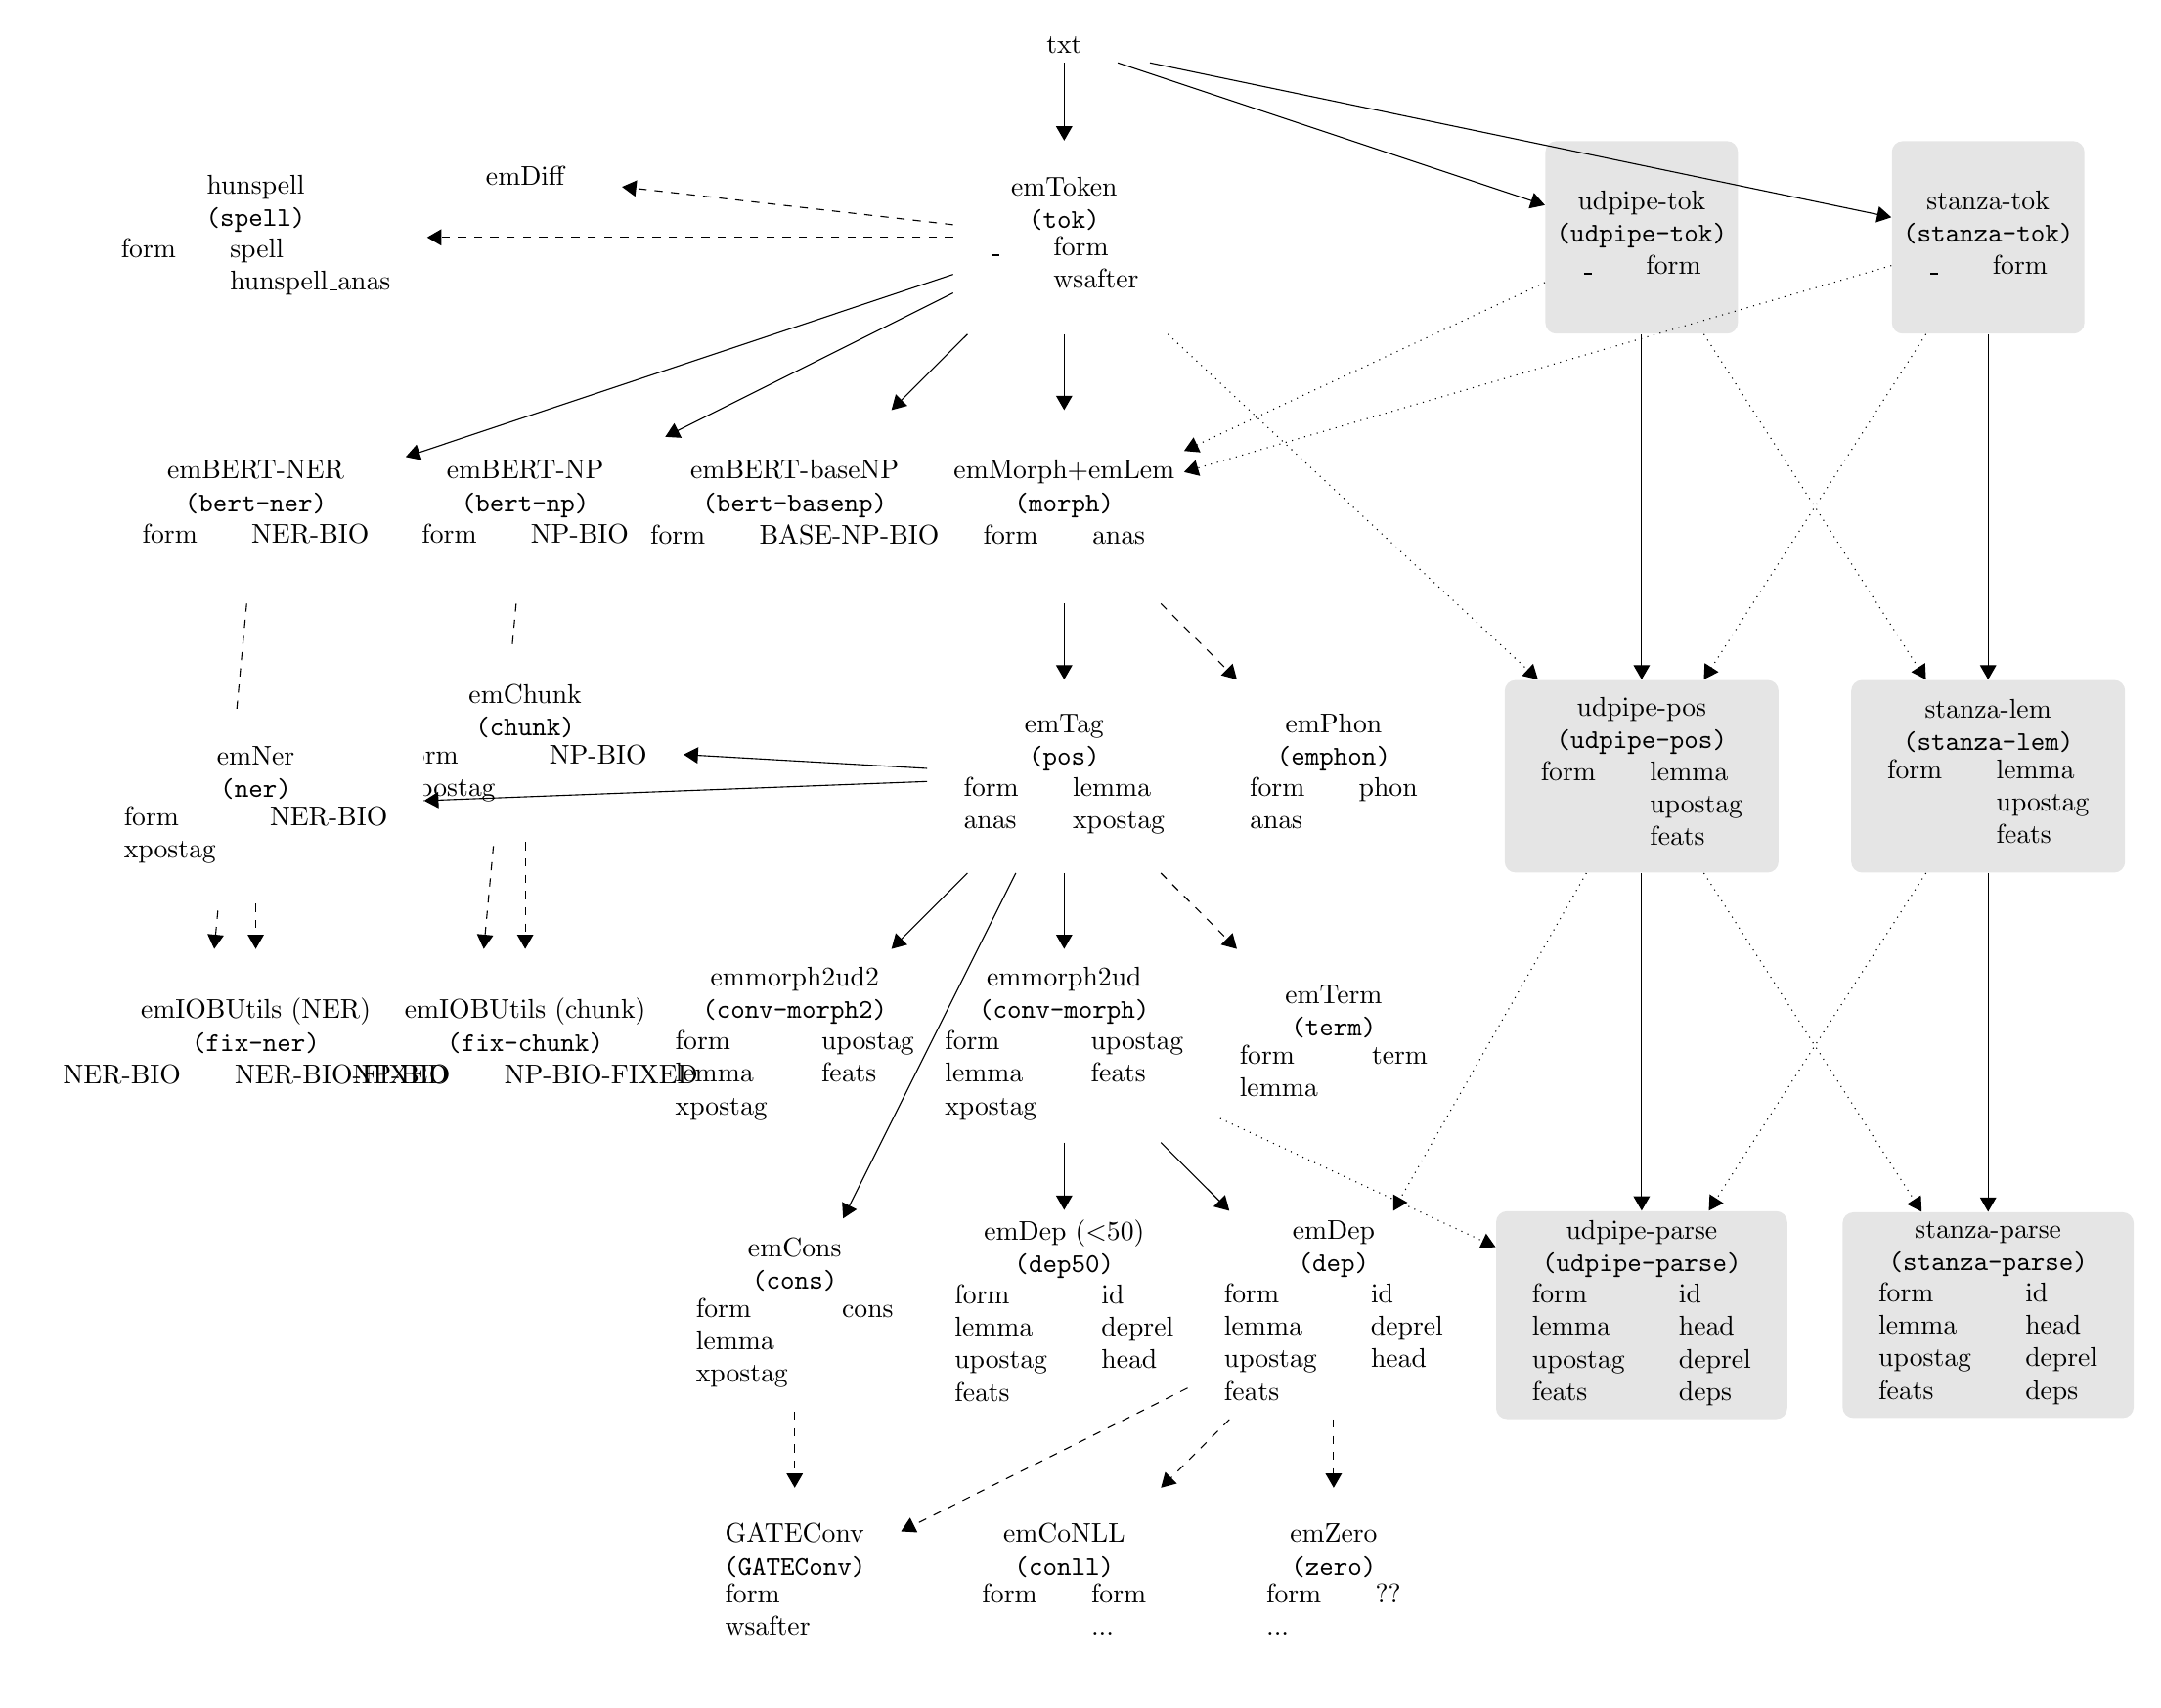
\begin{tikzpicture}[
      >=triangle 60,
      node distance = 3.5cm,
      start chain = going below,
      every node/.style = {rectangle, rounded corners, align=center, minimum width=2.5cm},
      module/.style = {minimum height=2.5cm},
      module2/.style = {minimum height=2.5cm, fill=black!10},
      txt/.style = {fill=white, draw=white},
                    ]
\node (txt1)            [txt]                                       {txt};
%\node (txt2)            [txt, right of=txt1, xshift=4cm]           {txt};
% \node (txt3)            [txt, right of=txt2]           {txt};
\node (emtoken)         [module, below of=txt1, yshift=1cm]                     {emToken \\
                                                                    \texttt{(tok)} \\
                                                                    \begin{tabular}{ll}
                                                                    \_ & form \\
                                                                     & wsafter \\
                                                                    \end{tabular}};
\node (emmorph_emlem)   [module, below of=emtoken]                  {emMorph+emLem \\
                                                                    \texttt{(morph)} \\
                                                                    \begin{tabular}{ll}
                                                                    form & anas \\
                                                                    \end{tabular}};
\node (emtag)           [module, below of=emmorph_emlem]            {emTag \\
                                                                    \texttt{(pos)} \\
                                                                    \begin{tabular}{ll}
                                                                    form & lemma \\
                                                                    anas & xpostag \\
                                                                    \end{tabular}};
\node (emphon)          [module, right of=emtag]                    {emPhon \\
                                                                    \texttt{(emphon)} \\
                                                                    \begin{tabular}{ll}
                                                                    form & phon \\
                                                                    anas &  \\
                                                                    \end{tabular}};
\node (emmorph2ud)      [module, below of=emtag]                    {emmorph2ud \\
                                                                    \texttt{(conv-morph)} \\
                                                                    \begin{tabular}{ll}
                                                                    form & upostag \\
                                                                    lemma & feats \\
                                                                    xpostag & \\
                                                                    \end{tabular}};
\node (emmorph2ud2)     [module, left of=emmorph2ud]               {emmorph2ud2 \\
                                                                    \texttt{(conv-morph2)} \\
                                                                    \begin{tabular}{ll}
                                                                    form & upostag \\
                                                                    lemma & feats \\
                                                                    xpostag & \\
                                                                    \end{tabular}};
\node (emdep50)      [module, below of=emmorph2ud]          {emDep (\textless50)\\
                                                                    \texttt{(dep50)} \\
                                                                    \begin{tabular}{ll}
                                                                    form & id \\
                                                                    lemma & deprel \\
                                                                    upostag & head \\
                                                                    feats & \\
                                                                    \end{tabular}};
\node (emdep)           [module, right of=emdep50]               {emDep \\
                                                                    \texttt{(dep)} \\
                                                                    \begin{tabular}{ll}
                                                                    form & id \\
                                                                    lemma & deprel \\
                                                                    upostag & head \\
                                                                    feats & \\
                                                                    \end{tabular}};

\node (emcons)          [module, left of=emdep50]                    {emCons \\
                                                                    \texttt{(cons)} \\
                                                                    \begin{tabular}{ll}
                                                                    form & cons \\
                                                                    lemma &  \\
                                                                    xpostag & \\
                                                                    \end{tabular}};
\node (embert_basenp)   [module, left of=emmorph_emlem]            {emBERT-baseNP \\
                                                                    \texttt{(bert-basenp)} \\
                                                                    \begin{tabular}{ll}
                                                                    form & BASE-NP-BIO \\
                                                                    \end{tabular}};
\node (embert_np)       [module, left of=embert_basenp]            {emBERT-NP \\
                                                                    \texttt{(bert-np)} \\
                                                                    \begin{tabular}{ll}
                                                                    form & NP-BIO \\
                                                                    \end{tabular}};
\node (embert_ner)      [module, left of=embert_np]                {emBERT-NER \\
                                                                    \texttt{(bert-ner)} \\
                                                                    \begin{tabular}{ll}
                                                                    form & NER-BIO \\
                                                                    \end{tabular}};
\node (emchunk)         [module, below of=embert_np, yshift=4mm, fill=white]                   {emChunk \\
                                                                    \texttt{(chunk)} \\
                                                                    \begin{tabular}{ll}
                                                                    form & NP-BIO \\
                                                                    xpostag & \\
                                                                    \end{tabular}};
\node (emner)           [module, below of=embert_ner, yshift=-4mm, fill=white]                   {emNer \\
                                                                    \texttt{(ner)} \\
                                                                    \begin{tabular}{ll}
                                                                    form & NER-BIO \\
                                                                    xpostag & \\
                                                                    \end{tabular}};
\node (emIOBUtils_chunk)           [module, below of=emchunk, yshift=-4mm]                   {emIOBUtils (chunk) \\
                                                                    \texttt{(fix-chunk)} \\
                                                                    \begin{tabular}{ll}
                                                                    NP-BIO & NP-BIO-FIXED \\
                                                                    \end{tabular}};
\node (emIOBUtils_ner)           [module, below of=emner, yshift=4mm]                   {emIOBUtils (NER) \\
                                                                    \texttt{(fix-ner)} \\
                                                                    \begin{tabular}{ll}
                                                                    NER-BIO & NER-BIO-FIXED \\
                                                                    \end{tabular}};
\node (emdiff)          [module, above of=embert_np, yshift=8mm]                 {emDiff};
\node (hunspell)        [module, above of=embert_ner]            {hunspell \\
                                                                    \texttt{(spell)} \\
                                                                    \begin{tabular}{ll}
                                                                    form & spell \\
                                                                     & hunspell\_anas\\
                                                                    \end{tabular}};

\node (emterm)          [module, right of=emmorph2ud]               {emTerm \\
                                                                    \texttt{(term)} \\
                                                                    \begin{tabular}{ll}
                                                                    form & term \\
                                                                    lemma & \\
                                                                    \end{tabular}};

\node (emzero)          [module, below of=emdep]                    {emZero \\
                                                                    \texttt{(zero)} \\
                                                                    \begin{tabular}{ll}
                                                                    form & ?? \\
                                                                    ... & \\
                                                                    \end{tabular}};
\node (emconll)         [module, left of=emzero]                   {emCoNLL \\
                                                                    \texttt{(conll)} \\
                                                                    \begin{tabular}{ll}
                                                                    form & form \\
                                                                     & ... \\
                                                                    \end{tabular}};
\node (GATEConv)         [module, left of=emconll]                   {GATEConv \\
                                                                    \texttt{(GATEConv)} \\
                                                                    \begin{tabular}{ll}
                                                                    form & \\
                                                                    wsafter &
                                                                    \end{tabular}};

\node (udpipe-tok)      [module2, , right of=emtoken, xshift=4cm]   {udpipe-tok \\
                                                                    \texttt{(udpipe-tok)} \\
                                                                    \begin{tabular}{ll}
                                                                    \_ & form \\
                                                                    \end{tabular}};
\node (udpipe-pos)      [module2, below of=udpipe-tok, yshift=-3.5cm]               {udpipe-pos \\
                                                                    \texttt{(udpipe-pos)} \\
                                                                    \begin{tabular}{ll}
                                                                    form & lemma \\
                                                                     & upostag \\
                                                                     & feats \\
                                                                    \end{tabular}};
\node (udpipe-parse)    [module2, below of=udpipe-pos, yshift=-3.5cm]              {udpipe-parse \\
                                                                    \texttt{(udpipe-parse)} \\
                                                                    \begin{tabular}{ll}
                                                                    form & id \\
                                                                    lemma & head \\
                                                                    upostag & deprel \\
                                                                    feats & deps \\
                                                                    \end{tabular}};

\node (stanza-tok)      [module2, right of=udpipe-tok, xshift=1cm]        {stanza-tok \\
                                                                    \texttt{(stanza-tok)} \\
                                                                    \begin{tabular}{ll}
                                                                    \_ & form \\
                                                                    \end{tabular}};
\node (stanza-lem)      [module2, below of=stanza-tok, yshift=-3.5cm]               {stanza-lem \\
                                                                    \texttt{(stanza-lem)} \\
                                                                    \begin{tabular}{ll}
                                                                    form & lemma \\
                                                                     & upostag \\
                                                                     & feats \\
                                                                    \end{tabular}};
\node (stanza-parse)    [module2, below of=stanza-lem, yshift=-3.5cm]              {stanza-parse \\
                                                                    \texttt{(stanza-parse)} \\
                                                                    \begin{tabular}{ll}
                                                                    form & id \\
                                                                    lemma & head \\
                                                                    upostag & deprel \\
                                                                    feats & deps \\
                                                                    \end{tabular}};

\draw[->]   (txt1)          --  (emtoken);
\draw[->]   (txt1)          --  (udpipe-tok);
\draw[->]   (txt1)          --  (stanza-tok);

\draw[->]   (emtoken)       --  (emmorph_emlem);
\draw[->]   (emmorph_emlem) --  (emtag);
\draw[->]   (emtag)         --  (emmorph2ud);
\draw[->]   (emmorph2ud)    --  (emdep);
\draw[->]   (emmorph2ud)    --  (emdep50);
\draw[->]   (emtag)         --  (emmorph2ud2);
\draw[->]   (emtag)         --  (emcons);
\draw[->]   (emtag)         --  (emchunk);
\draw[->]   (emtag)         --  (emner);
\draw[->]   (emtoken)       --  (embert_basenp);
\draw[->]   (emtoken)       --  (embert_np);
\draw[->]   (emtoken)       --  (embert_ner);

\draw[dashed,->]   (emmorph_emlem)       --  (emphon);
\draw[dashed,->]   (emtoken)       --  (hunspell);
\draw[dashed,->]   (emtoken)       --  (emdiff);
\draw[dashed,->]   (emtag)       --  (emterm);
\draw[dashed,->]   (emcons)       --  (GATEConv);
\draw[dashed,->]   (emdep)       --  (GATEConv);
\draw[dashed,->]   (emdep)       --  (emconll);
\draw[dashed,->]   (emdep)       --  (emzero);

\draw[dashed,->]   (emner)       --  (emIOBUtils_ner);
\draw[dashed,->]   (emchunk)       --  (emIOBUtils_chunk);
\begin{pgfonlayer}{bg}
\draw[dashed,->]   ([xshift=-3cm]embert_ner)      --  (emIOBUtils_ner);
\draw[dashed,->]   ([xshift=-3cm]embert_np)       --  (emIOBUtils_chunk);
\end{pgfonlayer}

\draw[->]   (udpipe-tok)       --  (udpipe-pos);
\draw[->]   (udpipe-pos)       --  (udpipe-parse);

\draw[->]   (stanza-tok)       --  (stanza-lem);
\draw[->]   (stanza-lem)       --  (stanza-parse);

\draw[dotted,->]   (udpipe-tok)    --  (emmorph_emlem);
\draw[dotted,->]   (stanza-tok)    --  (emmorph_emlem);
\draw[dotted,->]   (emtoken)    --  (udpipe-pos);
\draw[dotted,->]   (udpipe-pos)    --  (emdep);
\draw[dotted,->]   (emmorph2ud)    --  (udpipe-parse);

\draw[dotted,->]   (udpipe-tok)    --  (stanza-lem);
\draw[dotted,->]   (udpipe-pos)    --  (stanza-parse);

\draw[dotted,->]   (stanza-tok)    --  (udpipe-pos);
\draw[dotted,->]   (stanza-lem)    --  (udpipe-parse);


;
\end{tikzpicture}
\end{document}